\documentclass[10pt]{exam}
\usepackage[hon]{template-for-exam}
\usepackage{tikz}
\usetikzlibrary{shadings,decorations.pathmorphing,arrows.meta,patterns}


\title{Multi-Body Problem (Consolidation)}
\author{Rohrbach}
\date{\today}

\begin{document}
\maketitle


\noindent
Two masses are suspended at rest.  Assume that $m_1=5.2$~kg and $m_2 = 1.7$~kg.
\begin{center}
  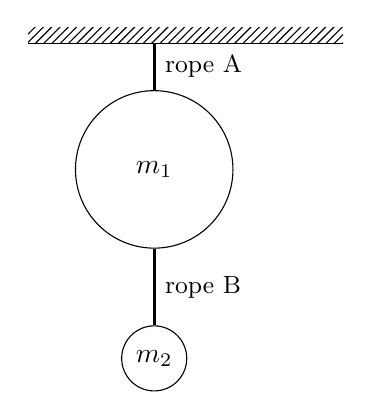
\begin{tikzpicture}[scale=0.8]
    \node[circle,draw,minimum size=2cm] (one) at (0,-2) {$m_1$};
    \node[circle,draw] (two) at (0,-5) {$m_2$};
    \draw[very thick] (one.south) -- (two.north) 
      node[midway,anchor=west] {\small rope B};
    \draw[very thick] (one.north) -- (0,0)
      node[midway,anchor=west] {\small rope A};
    \fill[pattern=north east lines] (-2,0) rectangle
      ++(5,0.25);
    \draw (-2,-0) -- ++(5,0);
  \end{tikzpicture}
\end{center}

\begin{parts}
  \part Calculate the tension on each rope. \vs
  \part Now you've detached rope A and are accelerating the system upward at a rate of \SI{0.5}{m/s^2}, what would be the tensions on both ropes? \vs
\end{parts}


  


\pagebreak
\noindent
Two boxes have masses $m_1=20$ kg and $m_2=10$ kg and are sitting on a frictionless surface connected by a massless cord. If they are pulled with an applied force of $F=50$ N, calculate (a) their acceleration and (b) the tension in the cord connecting them.


\tikzstyle{box}=[rounded corners,draw,minimum height=1cm,minimum width=1.5cm]

\begin{tikzpicture}
  \node[box] (one) at (0,0) {$m_1$};
  \node[box] (two) at (3,0) {$m_2$};
  \draw (one.east) -- (two.west);
  \draw[->,ultra thick] (two.east) ++(0,0.2) -- +(1,0) node[anchor=south west] {$\vec{F}$};
  \fill[pattern=north east lines] (-1,-0.5) rectangle ++(6,-0.25);
\end{tikzpicture}

\end{document}